\Exercise Troba l'error comès per aproximar el valor de $e^0.1$ a partir de l'aproximació lineal de la funció a l'origen. 
\label{ex:taylor1}
\Answer

Cal recordar que, en tant que infinitèssims equivalents,  $e^x \sim x+1$ per a valors de $x\rightarrow0$ (veure Figura \ref{fig:taylor1}).

\begin{center}
  \begin{minipage}{9cm}
  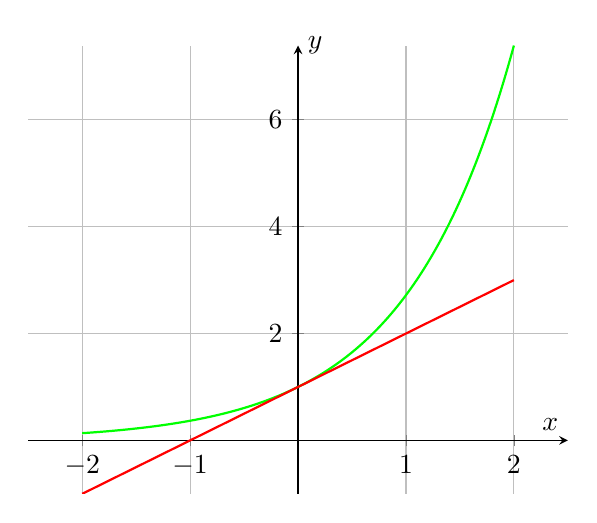
\begin{tikzpicture}[>=latex]
    \begin{axis}[%axis equal,
      axis lines=middle, 
      %xmin=-5, xmax=5,
      %ymin=-100, ymax=50,
      %xtick={-5,...,5},
      %ytick={-100,-50,0,50},
      grid=major,
      samples=222,
      xlabel={$x$},
      xlabel style = {anchor=south east},
      ylabel={$y$},
      ylabel style = {anchor=west},
      enlarge x limits={abs=0.5},
    ]
    \addplot[draw=green, thick, mark=none,domain=-2:2]{exp(x)}; 
    \addplot[draw=red, thick, mark=none,domain=-2:2]{x+1};
  
    \end{axis}
    \end{tikzpicture}
    \captionof{figure}{Les gràfiques de les funcions $y=e^x$ (verda) i $y=x+1$ (vermella) coincideixen en el seu valor i en la seva primera derivada al voltant de $x=0$ (són infinitèssims equivalents).}
    \label{fig:taylor1}
  \end{minipage} 
  \end{center}

  Per tant, per a valors propers a zero, com és el cas de $x=0.1$, teniom que
  \[e^{0.1} \sim 0.1 +1 = 1.1\]

  Podem comprovar amb la nostra calculadora que el valor correcte fins a 4 xifres decimals és $e^{0.1}=1.1052$.


\blacksquare 